% Instructions for Combinatorial Commutative Algebra style.

% CCA papers begin with the following two lines. 
\documentclass[12pt]{article}
\usepackage[amsmath]{cca}
% Omit the option "[amsmath]" if you do not want to use the amsmath package,
% or replace it with [mathtools] if you want to use the mathtools package.

% GEOMETRY
% The style file sets page size and margins, please remove any command
% or package that might change them (e.g. geometry, fullpage, etc.)

% PACKAGES
% Packages geometry, amssymb, amsthm, hyperref, microtype and enumitem are already loaded. 
% Please do not reload them or set any of their options.
% Forbidden packages:  fullpage, authblk, babel
% Load any additional packages and their options here. For example:
\usepackage{verbatim}
\usepackage{tikz}

% THEOREM ENVIRONMENTS
% Theorem-like environments that are declared in the style file are:
%   theorem, lemma, corollary, proposition, fact, observation, claim, note
%   definition, example, conjecture, open, problem, question, remark, notation

% CLEVEREF PACKAGE
% The cleveref package is sensitive to the order that packages are loaded,
% and is incompatible with some. If you use \usepackage{cleveref} yourself,
% it will probably not work properly (lemmas will be shown as theorems, etc.).
% The best way is to add it as an option to package cca, for example:
%    \usepackage[amsmath,cleveref]{cca}
% To pass options to the cleveref package you can do it like this:
%    \def\cleverefoptions{capitalize,noabbrev}
%    \usepackage[amsmath,cleveref]{cca}

% TITLE
% If needed, include a line break (\\) at an appropriate place in the title.
% Footnotes on titles are not allowed.
\title{Combinatorial Commutative Algebra:\\Style guidelines for authors}

% AUTHORS
% Autor information follows the following format:
% \author{Name}{Affiliation}{email}{website}
% Enter email as text: user@domain (do not use mailto:, url, or links)
% Website must be empty {} or text without http(s)://
% Please confirm links generated for emails and websites work as intended
\author{Ayşe First}{Department of Mathematics, University of the North\\Coldtown, YT, Canada}{first@email.edu}{example.org/~first}
\author{Elizabeth Second}{Department of Mathematics and Statistics, Universidade do Sul\\Rio de Janeiro, Brazil}{second@email.edu}{example.org/~second}
\author{Séraphine Third}{Department of Combinatorics and Optimization, Central College\\Centertown, OH, USA}{third@email.edu}{}
\author{Tomoaki Fourth}{Mathematics Department, Mountain Regional University\\Tokyo, Japan}{fourth@email.edu}{example.org/~fourth}
\author{Lina Q.~Fifth}{School of Mathematics, Seaside College\\Cape Town, South Africa}{fifth@email.edu}{example.org/~fifth}
\author{Zoë L.~Sixth}{Fictional Department, Imaginary University\\Realtown, United Kingdom}{sixth@email.edu}{}

% Information such as grant funding goes in the Acknowledgement
% section at the end of the paper, not in footnotes.
% Do not use the \thanks command.

% CCA restricts the use of footnotes, with two exceptions:
% 1) funding agencies that require acknowledgement on the first page of a publication,
% 2) corresponding authors that require acknowledgement for institutional purposes.
% In these cases, enter a number n (=1,2,3,etc) in the optional argument of \author.
% n is the footnote mark, text is entered as \authornote{n}{Footnote} later.
% The same n can be reused for more than one author.
% For example:
% \author[1]{First Author}{Affiliation}{email}{website}
% \author[1]{Second Author}{Affiliation}{email}{website}
% \authornote{1}{Footnote text for First and Second Author.}

% DATES
% Give the submission and acceptance dates in the format shown.
% The editors will insert the publication date in the third argument.
\dateline{Jan 1, 2026}{Jan 2, 2026}{TBD}

% SUBJECT CODES
% Give one or more subject codes separated by commas.
% Codes are available from https://mathscinet.ams.org/mathscinet/msc/msc2020.html
\MSC{05E40, 13F70}

% KEYWORDS
% Give 3 to 6 keywords separated by commas, singular is preferred
\keywords{combinatorics, algebra, commutative ring}

% COPYRIGHT AND LICENSE
% CCA leaves copyright with authors.
% Uncomment exactly one of the following copyright statements.

% For articles with a single author:  ==========================
%\Copyright{The author.}
%\Copyright{The author. Released under the \href{\CCBYURL}{CC BY license (International 4.0)}.}
%\Copyright{The author. Released under the \href{\CCBYNDURL}{CC BY-ND license (International 4.0)}.}
% For articles with more than one author: ======================
%\Copyright{The authors.}
\Copyright{The authors. Released under the \href{\CCBYURL}{CC BY license (International 4.0)}.}
%\Copyright{The authors. Released under the \href{\CCBYNDURL}{CC BY-ND license (International 4.0)}.}

% See https://creativecommons.org/licenses/ for a full explanation of the licenses.
% CCA recommends CC BY-ND or CC BY. Both these licenses allow others
% to freely distribute your work while giving credit to you. The difference
% between them is that CC BY-ND only allows distribution unchanged and in
% whole, while CC BY also allows remixing, tweaking and building upon your work.  


\begin{document}

\maketitle

\begin{tikzpicture}[remember picture,overlay,shift={(current page.north west)}]
\node[anchor=north west,xshift=0.5cm,yshift=-0.5cm]{
\includegraphics[width=1in]{CCAlogo.png}};
\end{tikzpicture}

% ABSTRACT
% A brief abstract must be included at the beginning of the submission.
% The abstract should provide context for the work and list new contributions.
% It should be self-contained and without references to the bibliography or
% other parts of the submission. The use of TeX code in the abstract is not
% recommended as the resulting text may not visualize correctly in a web browser;
% in particular, user-defined TeX macros must not be used in the abstract.

\begin{abstract}
  This note illustrates the main features of the style used for
  articles in the journal Combinatorial Commutative Algebra.  It also
  serves a style guideline for authors preparing publications for said
  journal.
\end{abstract}


\section{Introduction}

\textit{Combinatorial Commutative Algebra} (CCA) is a diamond
open-access journal run for and by mathematicians. It publishes
high-quality research at the interface of combinatorics and
commutative algebra and disseminates articles without fees or access
barriers.
    
Illustrative (non-exhaustive) topics of CCA include:
monomial/Stanley--Reisner/edge ideals; toric ideals and semigroup
rings; homological invariants and free resolutions; Lefschetz
properties; combinatorial topology and $f$-vectors; Gr\"obner/initial
ideals, determinantal/Schubert contexts; arrangements; tropical
geometry and related combinatorial Hodge theory; and applications
(e.g., coding theory, algebraic statistics).


\section{Preparing articles for CCA}

CCA accepts articles prepared using LaTeX. Publication versions will
be produced using a recent version of pdfLaTeX. CCA uses the style
file \verb|cca.sty| which can be downloaded at INSERT URL. Place this
file in the same directory as your article's TeX file to compile.


\subsection{Preamble and packages}

CCA articles begin with the following two lines.
\begin{verbatim}
\documentclass[12pt]{article}
\usepackage[amsmath]{cca}
\end{verbatim}
\begin{itemize}
\item The option \verb|amsmath| can be omitted, if the
  \texttt{amsmath} package is not needed, or replaced by
  \verb|mathtools|, if the \texttt{mathtools} package is used.  Both
  \texttt{amsmath} and \texttt{mathtools} are loaded with their
  default options.
\item The packages \texttt{geometry}, \texttt{amsthm},
  \texttt{amssymb}, \texttt{hyperref}, \texttt{microtype}, and
  \texttt{enumitem} are automatically loaded. Please do not reload or
  set any options for these packages.
\item The packages \texttt{fullpage}, \texttt{authblk}, \texttt{babel}
  are explicitly forbidden, as is any command that would change page
  or margin sizes.
\item The \texttt{tikz} package will be loaded at production to draw
  the journal logo. Any conflicts between \texttt{tikz} and other
  packages should be resolved beforehand.
\end{itemize}
   

\begin{note}
  To use the \texttt{cleveref} package add it as an option to the
  \texttt{cca} package as follows.
\begin{verbatim}
\usepackage[amsmath,cleveref]{cca}
\end{verbatim}
  Loading \texttt{cleveref} directly may cause it to improperly label
  environments.  Options for the \texttt{cleveref} package may be
  passed as in the following example.
\begin{verbatim}
\def\cleverefoptions{capitalize,noabbrev}
\usepackage[amsmath,cleveref]{cca}
\end{verbatim}
\end{note}


\subsection{Mandatory information}

All CCA submissions \textbf{must} contain the following information.

\begin{description}
\item[Title:] The title of the article is entered in the preamble
  using the command \verb|\title{}|. If necessary, a line break can be
  inserted using \verb|\\| as in
  \verb|\title{First line\\Second line}|.  Footnotes on titles are not
  allowed.
\item[Authors:] For each author, please enter their contact
  information in the preamble using the following command.
  \begin{center}
    \verb|\author{Name}{Affiliation\\Address}{email}{website}|
  \end{center}
  All arguments are mandatory, but the website argument can be empty.
  The email address should be entered as text without the
  \verb|mailto:| URI scheme. Similarly, the website, if any, should be
  entered as text without the \verb|http(s)://| protocol. Clickable
  links will be generated upon compilation for both email and website;
  please ensure these links work as intended. The author names are
  printed on the first page, while the author contact information is
  printed at the end by inserting the command
  \verb|\authorinformation| before \verb|\end{document}|.  Footnotes
on author names are prohibited, with two exceptions (see Note
\ref{footnotes}).
\item[Dates:] Authors may provide submission and acceptance dates in
  the preamble via
  \begin{center}
    \verb|\dateline{<Submitted>}{<Accepted>}{TBD}|;
  \end{center}
  production will fill in the publication date. Dates must be entered
  in the format ``Month Day, Year'', with month abbreviated to the
  first three letters (e.g.: Jan, Dec).
\item[Abstract:] A brief abstract must be included at the beginning of
  the submission.  The abstract should provide context for the work
  and list new contributions.  It should be self-contained and without
  references to the bibliography or other parts of the submission. The
  use of TeX code in the abstract is not recommended as the resulting
  text may not visualize correctly in a web browser; in particular,
  user-defined TeX macros must not be used in the abstract.  The
  abstract should be entered in an \verb|abstract| environment placed
  after the command \verb|\maketitle| at the beginning of the
  document.
\item[Subject Classifications:] Provide at least one 5-digit code from
  the
  \href{https://mathscinet.ams.org/mathscinet/msc/msc2020.html}{2020
    Mathematics Subject Classification}.  Additional codes should be
  separated by commas.
\item[Keywords:] Provide 3 to 6 keywords separated by commas. Keywords
  should be lowercase, except for proper names. Singular is preferred.
\item[Copyright:] Authors publishing in CCA retain copyright of their
  work.  CCA recommends using either the Creative Commons BY
  (Attribution) or BY-ND (Attribution-No Derivative) license. Both
  licenses allow others to freely distribute the work while giving
  proper credit to the authors.  The difference between the two
  licenses is that CC BY-ND only allows distribution unchanged and in
  whole, while CC BY also allows remixing, tweaking and building upon
  the original work.  The comments in the preamble of this file
  contain a few lines of text with various copyright options, such as:
  \begin{itemize}
  \item The authors.
  \item The authors. Released under the \href{\CCBYURL}{CC BY license
      (International 4.0)}.
  \item The authors. Released under the \href{\CCBYNDURL}{CC BY-ND
      license (International 4.0)}.
  \end{itemize}
  and equivalent versions for single-author papers. Authors should
  uncomment the single line corresponding to the license of their
  choice. Copyright information will be printed as a footnote to the
  first page, with a link to the details of the chosen CC license, if
  any.
\end{description}

\begin{note}\label{footnotes}
  Other than copyright information, CCA restricts the use of
  footnotes, including on title and author names; in particular, the
  command \verb|\thanks| is forbidden. There are two exceptions.
  \begin{enumerate}
  \item Funding that must be acknowledged on the first page of a
    publication by explicit requirement of the funding
    agency. Otherwise, funding should only be mentioned in the
    Acknowledgment section at the end of the article.
  \item Corresponding authors that require acknowledgement on the
    first page of a publication for institutional purposes. Otherwise,
    CCA does not recognize a corresponding author in published
    articles, even though such a role may be a part of the editorial
    tools used by CCA.
  \end{enumerate}
  In these cases, enter the required information as a footnote on your
  name by placing the following code in the preamble:
    \begin{verbatim}
    \author[n]{Name}{Affiliation\\Address}{email}{website}
    \authornote{n}{Footnote text}\end{verbatim}
  where \verb|n| is a positive integer starting at 1.
  The same footnote can be reused, for example,
  when two or more authors are funded by the same source.
  Increase \verb|n| by one for the next footnote.
\end{note}


\subsection{Document body}

\begin{itemize}
\item The document environment should start with \verb|\maketitle|
  followed by the abstract.
\item All sections should be automatically numbered. Do not include a
  table of contents.
\item The default font and font sizes are set by the \verb|cca.sty|
  file; please do not alter them.
\item Accented letters in names and text, such as Gröbner or Erdős,
  can be input directly as Unicode characters instead of LaTeX
  commands. For example, á can be used instead of \verb|\'a|.
\item The \verb|cca.sty| file defines the following environments:
  theorem, lemma, corollary, proposition, fact, observation, claim,
  note, definition, example, conjecture, open, problem, question,
  remark, notation.  The environments are numbered sequentially within
  sections.
\item Equations environments are also numbered within sections. If an
  equation is not referred to in the rest of the article, the
  numbering should be suppressed.
\item Figures and tables should always be included as floats within a
  figure and table environment respectively. All floats must be
  labeled, captioned, and are automatically numbered within sections.
  As the position of a float may change during production, please
  refer to it by label (e.g.: Figure \ref{fig:graph}) rather than
  using expressions such as the figure/table below/above.
\item In the interest of producing high quality figures, we strongly
  recommend creating images using the PGF/TikZ package and including
  code directly into your LaTeX file. As an alternative, authors may
  submit image files in PDF or EPS format, preferably containing
  vector graphics.
\end{itemize}


\subsection{Bibliographic references}

All CCA articles must include a complete and up-to-date list of
bibliographic references. Such information can usually be retrieved
from databases like \href{https://mathscinet.ams.org}{Mathscinet} and
\href{https://zbmath.org/}{zbMath}; the latter can also be used for
arXiv preprints. All references appearing in the bibliography must be
cited in the text. Please make citations as explicit as possible by
including an environment number (e.g.: Theorem 2.1(a), Example IV), a
(sub)section number, or a page number.  Upon compilation, backlinks
from the references to the text will be automatically inserted.

CCA recommends using BibTeX with the
\href{https://www.bibtex.com/s/bibliography-style-base-abbrv/}{\texttt{abbrv}
  bibliography style}, then copying and pasting the contents of the
compiled \texttt{.bbl} file into the main source file. If a dedicated
\texttt{.bib} is used for the submission, then it can be uploaded
along with the source file. If not using BibTeX, please use
\texttt{thebibliography} environment and format your references as
close as possible to the aforementioned \texttt{abbrv} style.

Whenever possible, CCA suggests adding arXiv and DOI links after each
reference inside \texttt{thebibliography} environment. For arXiv
papers, use \verb|\arxiv{YYMM.number}| or the appropriate
identifier. For published works, use \verb|\doi{number}|. See this
document and its source for examples.


\section{Sample content}

\begin{definition}
  A commutative ring is called \emph{amazing} if it is isomorphic to
  the edge ring of an amazing graph.
\end{definition}

\begin{example}
  The complete graph on five vertices (see Figure \ref{fig:graph}) is
  amazing. The fictional index of the graph can be found by solving
  for $f$ in
  \begin{equation}
    v-e+f=2,
  \end{equation}
  where $v$ is the number of vertices and $e$ is the number of edges.
\end{example}

\begin{figure}[htb]
  \centering
  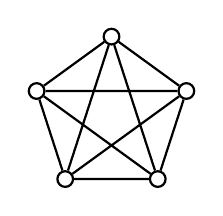
\begin{tikzpicture}
    \tikzset{vertex/.style = {shape=circle,draw,thick,inner sep=2pt}}
    \tikzset{edge/.style = {thick}} \node[vertex] (a) at (90:1) {};
    \node[vertex] (b) at (162:1) {}; \node[vertex] (c) at (234:1) {};
    \node[vertex] (d) at (306:1) {}; \node[vertex] (e) at (18:1) {};
    \draw[edge] (a) -- (b) -- (c) -- (d) -- (e) -- (a); \draw[edge]
    (a) -- (c) -- (e) -- (b) -- (d) -- (a);
  \end{tikzpicture}
  \caption{A complete graph on five vertices.}
  \label{fig:graph}
\end{figure}

\begin{theorem}
  Every amazing ring is excellent.
\end{theorem}

\begin{proof}
  It will be enough to show that an amazing graph is astounding since
  the edge ring of an astounding graph is excellent as shown in \dots
\end{proof}

The reader will find many interesting examples of the interactions
between combinatorics and commutative algebra in the vast literature
on the subject which includes works such as
\cite{zbMATH00922152,zbMATH03545783,zbMATH00833410,zbMATH06413064}.


\section*{Acknowledgements}

Elizabeth Second was partially supported by Amazing Grant
\#1.  All authors wish to thank several people for useful
conversations.

%BIBLIOGRAPHY
% CCA recommends using BibTeX with the abbrv file, then copying and pasting
% the contents of the .bbl file below.
% If a dedicated .bib file is used, you may enter its name and uncomment
% the lines below, then upload the file along with your TeX source

% \bibliographystyle{abbrv}
% \bibliography{enter_name_of_bib_file}

% CCA also recommends using \doi{...} and \arxiv{...} as in the examples below,
% to produce clickable links to bibliographic sources

\begin{thebibliography}{1}
\bibitem{zbMATH00922152}
D.~Eisenbud and B.~Sturmfels.
\newblock Binomial ideals.
\newblock {\em Duke Math. J.}, 84(1):1--45, 1996.
\arxiv{alg-geom/9401001} \doi{10.1215/S0012-7094-96-08401-X}

\bibitem{zbMATH03545783}
M.~Hochster.
\newblock Cohen-Macaulay rings, combinatorics, and simplicial complexes.
\newblock Ring {Theory} {II}, {Proc}. 2nd {Okla}. {Conf}. 1975, 171-223, 1977.

\bibitem{zbMATH00833410}
R.~P. Stanley.
\newblock {\em Combinatorics and commutative algebra.}, volume~41 of {\em Prog. Math.}
\newblock Basel: Birkh{\"a}user, 2nd ed., 1996. \doi{10.1007/b139094}

\bibitem{zbMATH06413064}
R.~H. Villarreal.
\newblock {\em Monomial algebras}.
\newblock Monogr. Res. Notes Math. Boca Raton, FL: CRC Press, 2nd ed., 2015.
\doi{10.1201/b18224}

% If the backlink to your last citation appears as a separate paragraph,
% please leave an empty line before \end{thebibliography}
\end{thebibliography}


% the next command is required to print author contact
% information at the end of the paper
\authorinformation

% If the authors submit a corrigendum to their published manuscript, 
% the content of their corrigendum goes below. 
% For the date, please include the date of your corrigendum submission.

\corrigendum{Oct 11, 2026}

Author(s)  may submit a corrigendum if:
\begin{itemize}
\item the main result(s) remain true; and
\item author(s) can provide a corrected or replacement proof, or a
  precise amendment (e.g., added hypothesis, corrected bound) that
  preserves the paper’s core contributions.
\end{itemize}

If the error makes a central statement false, substantially weakens
the results beyond the paper’s scope, or requires extensive new
theory, the editors may instead pursue a retraction or invite a new,
standalone submission.


\subsection*{Communicating a Corrigendum to CCA}

To request a corrigendum, the author(s) should start a new submission
including the following information.

\begin{itemize}
\item A new section appended to the original paper by placing
  \begin{center}
    \verb|\corrigendum{Month Day, Year}|
  \end{center}
  immediately after \verb|\authorinformation| in the accepted
  manuscript’s source file (using cca style). The date is the day author(s) submit the
  corrigendum to the managing editors.  The corrigendum section must
  include an opening paragraph explaining:
  \begin{enumerate}[label=(\roman*)]
  \item the issue,
  \item why a correction/replacement proof is needed,
  \item which results are impacted by the changes.
  \end{enumerate}
\item For each correction: make sure to include the precise
  \emph{location} in the published version
  (section/theorem/equation/figure; page/line if helpful) and the
  \emph{corrected text/formula}.
\item If supplying a new proof for a theorem, restate the theorem, and
  provide a self-contained proof that introduces no new results and no
  renumbering (unless the fix requires).
\end{itemize}


\subsection*{Review and outcome}
Corrigenda that include a replacement proof or change mathematical
content will be externally checked (preferably by the original
referee(s) or a subject expert), with the review focused on the
corrected portions unless broader interaction is required.

Upon a positive check, the corrigendum is appended to the published
PDF and the article page notes “A corrigendum was added on [date]”;
the DOI and record remain unchanged.


\end{document}
